% Created by tikzDevice version 0.6.2 on 2012-03-05 20:59:05
% !TEX encoding = UTF-8 Unicode
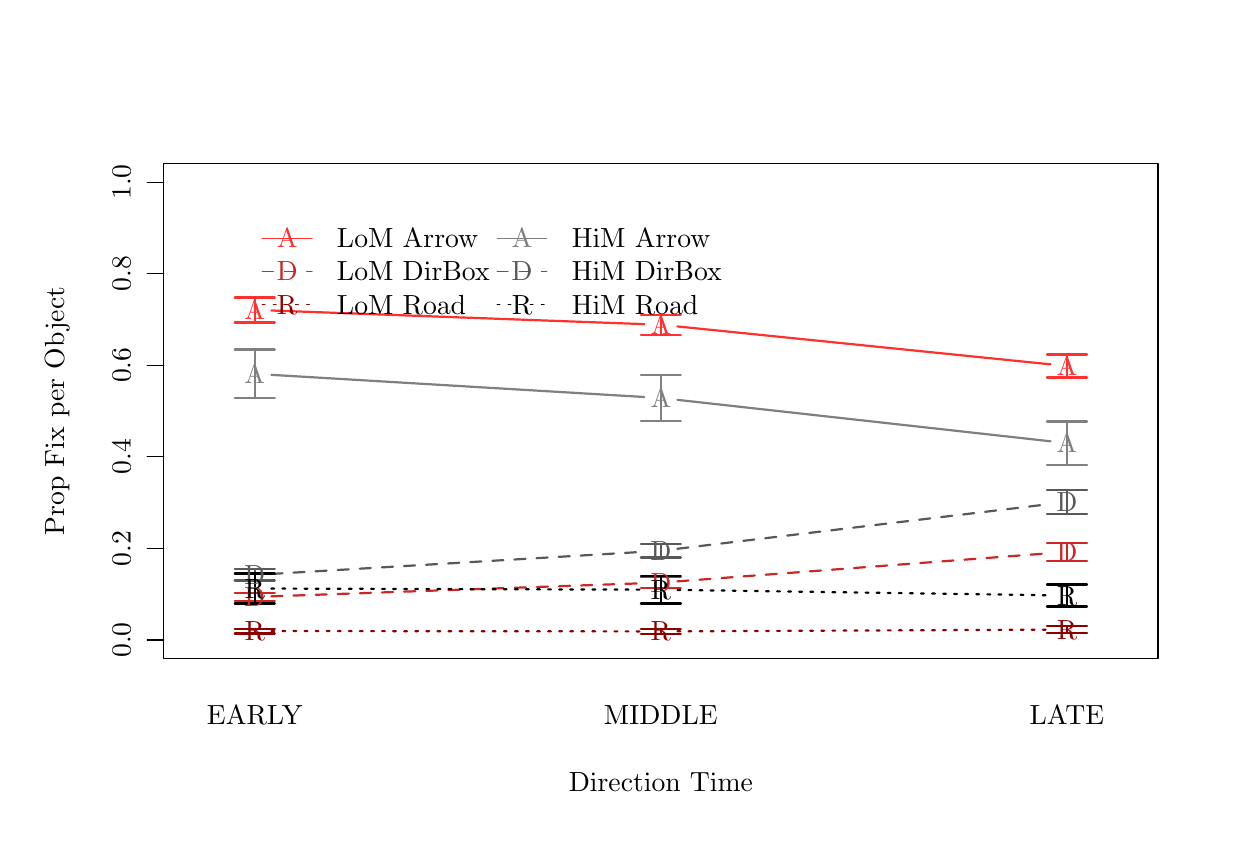
\begin{tikzpicture}[x=1pt,y=1pt]
\definecolor[named]{drawColor}{rgb}{0.00,0.00,0.00}
\definecolor[named]{fillColor}{rgb}{1.00,1.00,1.00}
\fill[color=fillColor,fill opacity=0.00,] (0,0) rectangle (433.62,289.08);
\begin{scope}
\path[clip] ( 49.20, 61.20) rectangle (408.42,239.88);
\definecolor[named]{fillColor}{rgb}{0.00,0.00,0.00}
\definecolor[named]{drawColor}{rgb}{1.00,0.19,0.19}

\draw[color=drawColor,line width= 0.8pt,line cap=round,line join=round,fill opacity=0.00,] ( 88.07,186.88) -- (222.81,181.95);

\draw[color=drawColor,line width= 0.8pt,line cap=round,line join=round,fill opacity=0.00,] (234.78,181.12) -- (369.58,167.42);
\end{scope}
\begin{scope}
\path[clip] (  0.00,  0.00) rectangle (433.62,289.08);
\definecolor[named]{fillColor}{rgb}{0.00,0.00,0.00}
\definecolor[named]{drawColor}{rgb}{0.00,0.00,0.00}

\draw[color=drawColor,line cap=round,line join=round,fill opacity=0.00,] ( 49.20, 67.82) -- ( 49.20,233.26);

\draw[color=drawColor,line cap=round,line join=round,fill opacity=0.00,] ( 49.20, 67.82) -- ( 43.20, 67.82);

\draw[color=drawColor,line cap=round,line join=round,fill opacity=0.00,] ( 49.20,100.91) -- ( 43.20,100.91);

\draw[color=drawColor,line cap=round,line join=round,fill opacity=0.00,] ( 49.20,134.00) -- ( 43.20,134.00);

\draw[color=drawColor,line cap=round,line join=round,fill opacity=0.00,] ( 49.20,167.08) -- ( 43.20,167.08);

\draw[color=drawColor,line cap=round,line join=round,fill opacity=0.00,] ( 49.20,200.17) -- ( 43.20,200.17);

\draw[color=drawColor,line cap=round,line join=round,fill opacity=0.00,] ( 49.20,233.26) -- ( 43.20,233.26);

\node[rotate= 90.00,color=drawColor,anchor=base,inner sep=0pt, outer sep=0pt, scale=  1.00] at ( 37.20, 67.82) {0.0};

\node[rotate= 90.00,color=drawColor,anchor=base,inner sep=0pt, outer sep=0pt, scale=  1.00] at ( 37.20,100.91) {0.2};

\node[rotate= 90.00,color=drawColor,anchor=base,inner sep=0pt, outer sep=0pt, scale=  1.00] at ( 37.20,134.00) {0.4};

\node[rotate= 90.00,color=drawColor,anchor=base,inner sep=0pt, outer sep=0pt, scale=  1.00] at ( 37.20,167.08) {0.6};

\node[rotate= 90.00,color=drawColor,anchor=base,inner sep=0pt, outer sep=0pt, scale=  1.00] at ( 37.20,200.17) {0.8};

\node[rotate= 90.00,color=drawColor,anchor=base,inner sep=0pt, outer sep=0pt, scale=  1.00] at ( 37.20,233.26) {1.0};

\draw[color=drawColor,line cap=round,line join=round,fill opacity=0.00,] ( 49.20, 61.20) --
	(408.42, 61.20) --
	(408.42,239.88) --
	( 49.20,239.88) --
	( 49.20, 61.20);
\end{scope}
\begin{scope}
\path[clip] (  0.00,  0.00) rectangle (433.62,289.08);
\definecolor[named]{fillColor}{rgb}{0.00,0.00,0.00}
\definecolor[named]{drawColor}{rgb}{0.00,0.00,0.00}

\node[color=drawColor,anchor=base,inner sep=0pt, outer sep=0pt, scale=  1.00] at (228.81, 13.20) {Direction Time};

\node[rotate= 90.00,color=drawColor,anchor=base,inner sep=0pt, outer sep=0pt, scale=  1.00] at ( 13.20,150.54) {Prop Fix per Object};
\end{scope}
\begin{scope}
\path[clip] ( 49.20, 61.20) rectangle (408.42,239.88);
\definecolor[named]{fillColor}{rgb}{0.00,0.00,0.00}
\definecolor[named]{drawColor}{rgb}{0.80,0.15,0.15}

\draw[color=drawColor,line width= 0.8pt,dash pattern=on 4pt off 4pt ,line cap=round,line join=round,fill opacity=0.00,] ( 88.07, 83.59) -- (222.81, 88.34);

\draw[color=drawColor,line width= 0.8pt,dash pattern=on 4pt off 4pt ,line cap=round,line join=round,fill opacity=0.00,] (234.79, 89.00) -- (369.57, 99.19);
\definecolor[named]{drawColor}{rgb}{0.55,0.00,0.00}

\draw[color=drawColor,line width= 0.8pt,dash pattern=on 1pt off 3pt ,line cap=round,line join=round,fill opacity=0.00,] ( 88.07, 71.06) -- (222.81, 70.92);

\draw[color=drawColor,line width= 0.8pt,dash pattern=on 1pt off 3pt ,line cap=round,line join=round,fill opacity=0.00,] (234.81, 70.94) -- (369.55, 71.56);
\definecolor[named]{drawColor}{rgb}{0.50,0.50,0.50}

\draw[color=drawColor,line width= 0.8pt,line cap=round,line join=round,fill opacity=0.00,] ( 88.06,163.63) -- (222.82,155.62);

\draw[color=drawColor,line width= 0.8pt,line cap=round,line join=round,fill opacity=0.00,] (234.77,154.60) -- (369.59,139.62);
\definecolor[named]{drawColor}{rgb}{0.35,0.35,0.35}

\draw[color=drawColor,line width= 0.8pt,dash pattern=on 4pt off 4pt ,line cap=round,line join=round,fill opacity=0.00,] ( 88.06, 91.68) -- (222.82, 99.70);

\draw[color=drawColor,line width= 0.8pt,dash pattern=on 4pt off 4pt ,line cap=round,line join=round,fill opacity=0.00,] (234.77,100.78) -- (369.59,116.97);
\definecolor[named]{drawColor}{rgb}{0.00,0.00,0.00}

\draw[color=drawColor,line width= 0.8pt,dash pattern=on 1pt off 3pt ,line cap=round,line join=round,fill opacity=0.00,] ( 88.07, 86.40) -- (222.81, 86.01);

\draw[color=drawColor,line width= 0.8pt,dash pattern=on 1pt off 3pt ,line cap=round,line join=round,fill opacity=0.00,] (234.81, 85.91) -- (369.55, 83.98);
\end{scope}
\begin{scope}
\path[clip] (  0.00,  0.00) rectangle (433.62,289.08);
\definecolor[named]{fillColor}{rgb}{0.00,0.00,0.00}
\definecolor[named]{drawColor}{rgb}{0.00,0.00,0.00}

\node[color=drawColor,anchor=base,inner sep=0pt, outer sep=0pt, scale=  1.00] at ( 82.07, 37.20) {EARLY};

\node[color=drawColor,anchor=base,inner sep=0pt, outer sep=0pt, scale=  1.00] at (228.81, 37.20) {MIDDLE};

\node[color=drawColor,anchor=base,inner sep=0pt, outer sep=0pt, scale=  1.00] at (375.55, 37.20) {LATE};
\end{scope}
\begin{scope}
\path[clip] (  0.00,  0.00) rectangle (433.62,289.08);
\definecolor[named]{fillColor}{rgb}{0.00,0.00,0.00}
\definecolor[named]{drawColor}{rgb}{0.00,0.00,0.00}

\node[color=drawColor,anchor=base west,inner sep=0pt, outer sep=0pt, scale=  1.00] at (390.22,223.32) {   };
\end{scope}
\begin{scope}
\path[clip] ( 49.20, 61.20) rectangle (408.42,239.88);
\definecolor[named]{fillColor}{rgb}{0.00,0.00,0.00}
\definecolor[named]{drawColor}{rgb}{1.00,0.19,0.19}

\draw[color=drawColor,line width= 0.8pt,line cap=round,line join=round,fill opacity=0.00,] ( 82.07,182.58) -- ( 82.07,191.61);

\draw[color=drawColor,line width= 0.8pt,line cap=round,line join=round,fill opacity=0.00,] ( 74.84,182.58) --
	( 82.07,182.58) --
	( 89.30,182.58);

\draw[color=drawColor,line width= 0.8pt,line cap=round,line join=round,fill opacity=0.00,] ( 89.30,191.61) --
	( 82.07,191.61) --
	( 74.84,191.61);

\draw[color=drawColor,line width= 0.8pt,line cap=round,line join=round,fill opacity=0.00,] (228.81,178.09) -- (228.81,185.38);

\draw[color=drawColor,line width= 0.8pt,line cap=round,line join=round,fill opacity=0.00,] (221.58,178.09) --
	(228.81,178.09) --
	(236.04,178.09);

\draw[color=drawColor,line width= 0.8pt,line cap=round,line join=round,fill opacity=0.00,] (236.04,185.38) --
	(228.81,185.38) --
	(221.58,185.38);

\draw[color=drawColor,line width= 0.8pt,line cap=round,line join=round,fill opacity=0.00,] (375.55,162.68) -- (375.55,170.94);

\draw[color=drawColor,line width= 0.8pt,line cap=round,line join=round,fill opacity=0.00,] (368.32,162.68) --
	(375.55,162.68) --
	(382.78,162.68);

\draw[color=drawColor,line width= 0.8pt,line cap=round,line join=round,fill opacity=0.00,] (382.78,170.94) --
	(375.55,170.94) --
	(368.32,170.94);
\definecolor[named]{drawColor}{rgb}{0.80,0.15,0.15}

\draw[color=drawColor,line width= 0.8pt,line cap=round,line join=round,fill opacity=0.00,] ( 82.07, 82.01) -- ( 82.07, 84.75);

\draw[color=drawColor,line width= 0.8pt,line cap=round,line join=round,fill opacity=0.00,] ( 74.84, 82.01) --
	( 82.07, 82.01) --
	( 89.30, 82.01);

\draw[color=drawColor,line width= 0.8pt,line cap=round,line join=round,fill opacity=0.00,] ( 89.30, 84.75) --
	( 82.07, 84.75) --
	( 74.84, 84.75);

\draw[color=drawColor,line width= 0.8pt,line cap=round,line join=round,fill opacity=0.00,] (228.81, 86.63) -- (228.81, 90.47);

\draw[color=drawColor,line width= 0.8pt,line cap=round,line join=round,fill opacity=0.00,] (221.58, 86.63) --
	(228.81, 86.63) --
	(236.04, 86.63);

\draw[color=drawColor,line width= 0.8pt,line cap=round,line join=round,fill opacity=0.00,] (236.04, 90.47) --
	(228.81, 90.47) --
	(221.58, 90.47);

\draw[color=drawColor,line width= 0.8pt,line cap=round,line join=round,fill opacity=0.00,] (375.55, 96.47) -- (375.55,102.82);

\draw[color=drawColor,line width= 0.8pt,line cap=round,line join=round,fill opacity=0.00,] (368.32, 96.47) --
	(375.55, 96.47) --
	(382.78, 96.47);

\draw[color=drawColor,line width= 0.8pt,line cap=round,line join=round,fill opacity=0.00,] (382.78,102.82) --
	(375.55,102.82) --
	(368.32,102.82);
\definecolor[named]{drawColor}{rgb}{0.55,0.00,0.00}

\draw[color=drawColor,line width= 0.8pt,line cap=round,line join=round,fill opacity=0.00,] ( 82.07, 70.20) -- ( 82.07, 71.93);

\draw[color=drawColor,line width= 0.8pt,line cap=round,line join=round,fill opacity=0.00,] ( 74.84, 70.20) --
	( 82.07, 70.20) --
	( 89.30, 70.20);

\draw[color=drawColor,line width= 0.8pt,line cap=round,line join=round,fill opacity=0.00,] ( 89.30, 71.93) --
	( 82.07, 71.93) --
	( 74.84, 71.93);

\draw[color=drawColor,line width= 0.8pt,line cap=round,line join=round,fill opacity=0.00,] (228.81, 69.96) -- (228.81, 71.86);

\draw[color=drawColor,line width= 0.8pt,line cap=round,line join=round,fill opacity=0.00,] (221.58, 69.96) --
	(228.81, 69.96) --
	(236.04, 69.96);

\draw[color=drawColor,line width= 0.8pt,line cap=round,line join=round,fill opacity=0.00,] (236.04, 71.86) --
	(228.81, 71.86) --
	(221.58, 71.86);

\draw[color=drawColor,line width= 0.8pt,line cap=round,line join=round,fill opacity=0.00,] (375.55, 70.39) -- (375.55, 72.79);

\draw[color=drawColor,line width= 0.8pt,line cap=round,line join=round,fill opacity=0.00,] (368.32, 70.39) --
	(375.55, 70.39) --
	(382.78, 70.39);

\draw[color=drawColor,line width= 0.8pt,line cap=round,line join=round,fill opacity=0.00,] (382.78, 72.79) --
	(375.55, 72.79) --
	(368.32, 72.79);
\definecolor[named]{drawColor}{rgb}{0.50,0.50,0.50}

\draw[color=drawColor,line width= 0.8pt,line cap=round,line join=round,fill opacity=0.00,] ( 82.07,155.17) -- ( 82.07,172.80);

\draw[color=drawColor,line width= 0.8pt,line cap=round,line join=round,fill opacity=0.00,] ( 74.84,155.17) --
	( 82.07,155.17) --
	( 89.30,155.17);

\draw[color=drawColor,line width= 0.8pt,line cap=round,line join=round,fill opacity=0.00,] ( 89.30,172.80) --
	( 82.07,172.80) --
	( 74.84,172.80);

\draw[color=drawColor,line width= 0.8pt,line cap=round,line join=round,fill opacity=0.00,] (228.81,147.09) -- (228.81,163.44);

\draw[color=drawColor,line width= 0.8pt,line cap=round,line join=round,fill opacity=0.00,] (221.58,147.09) --
	(228.81,147.09) --
	(236.04,147.09);

\draw[color=drawColor,line width= 0.8pt,line cap=round,line join=round,fill opacity=0.00,] (236.04,163.44) --
	(228.81,163.44) --
	(221.58,163.44);

\draw[color=drawColor,line width= 0.8pt,line cap=round,line join=round,fill opacity=0.00,] (375.55,131.17) -- (375.55,146.75);

\draw[color=drawColor,line width= 0.8pt,line cap=round,line join=round,fill opacity=0.00,] (368.32,131.17) --
	(375.55,131.17) --
	(382.78,131.17);

\draw[color=drawColor,line width= 0.8pt,line cap=round,line join=round,fill opacity=0.00,] (382.78,146.75) --
	(375.55,146.75) --
	(368.32,146.75);
\definecolor[named]{drawColor}{rgb}{0.35,0.35,0.35}

\draw[color=drawColor,line width= 0.8pt,line cap=round,line join=round,fill opacity=0.00,] ( 82.07, 89.29) -- ( 82.07, 93.36);

\draw[color=drawColor,line width= 0.8pt,line cap=round,line join=round,fill opacity=0.00,] ( 74.84, 89.29) --
	( 82.07, 89.29) --
	( 89.30, 89.29);

\draw[color=drawColor,line width= 0.8pt,line cap=round,line join=round,fill opacity=0.00,] ( 89.30, 93.36) --
	( 82.07, 93.36) --
	( 74.84, 93.36);

\draw[color=drawColor,line width= 0.8pt,line cap=round,line join=round,fill opacity=0.00,] (228.81, 97.60) -- (228.81,102.52);

\draw[color=drawColor,line width= 0.8pt,line cap=round,line join=round,fill opacity=0.00,] (221.58, 97.60) --
	(228.81, 97.60) --
	(236.04, 97.60);

\draw[color=drawColor,line width= 0.8pt,line cap=round,line join=round,fill opacity=0.00,] (236.04,102.52) --
	(228.81,102.52) --
	(221.58,102.52);

\draw[color=drawColor,line width= 0.8pt,line cap=round,line join=round,fill opacity=0.00,] (375.55,113.26) -- (375.55,122.11);

\draw[color=drawColor,line width= 0.8pt,line cap=round,line join=round,fill opacity=0.00,] (368.32,113.26) --
	(375.55,113.26) --
	(382.78,113.26);

\draw[color=drawColor,line width= 0.8pt,line cap=round,line join=round,fill opacity=0.00,] (382.78,122.11) --
	(375.55,122.11) --
	(368.32,122.11);
\definecolor[named]{drawColor}{rgb}{0.00,0.00,0.00}

\draw[color=drawColor,line width= 0.8pt,line cap=round,line join=round,fill opacity=0.00,] ( 82.07, 80.99) -- ( 82.07, 91.84);

\draw[color=drawColor,line width= 0.8pt,line cap=round,line join=round,fill opacity=0.00,] ( 74.84, 80.99) --
	( 82.07, 80.99) --
	( 89.30, 80.99);

\draw[color=drawColor,line width= 0.8pt,line cap=round,line join=round,fill opacity=0.00,] ( 89.30, 91.84) --
	( 82.07, 91.84) --
	( 74.84, 91.84);

\draw[color=drawColor,line width= 0.8pt,line cap=round,line join=round,fill opacity=0.00,] (228.81, 80.97) -- (228.81, 91.01);

\draw[color=drawColor,line width= 0.8pt,line cap=round,line join=round,fill opacity=0.00,] (221.58, 80.97) --
	(228.81, 80.97) --
	(236.04, 80.97);

\draw[color=drawColor,line width= 0.8pt,line cap=round,line join=round,fill opacity=0.00,] (236.04, 91.01) --
	(228.81, 91.01) --
	(221.58, 91.01);

\draw[color=drawColor,line width= 0.8pt,line cap=round,line join=round,fill opacity=0.00,] (375.55, 79.93) -- (375.55, 87.85);

\draw[color=drawColor,line width= 0.8pt,line cap=round,line join=round,fill opacity=0.00,] (368.32, 79.93) --
	(375.55, 79.93) --
	(382.78, 79.93);

\draw[color=drawColor,line width= 0.8pt,line cap=round,line join=round,fill opacity=0.00,] (382.78, 87.85) --
	(375.55, 87.85) --
	(368.32, 87.85);
\definecolor[named]{drawColor}{rgb}{1.00,0.19,0.19}

\node[color=drawColor,anchor=base,inner sep=0pt, outer sep=0pt, scale=  1.00] at ( 82.07,183.65) {A};

\node[color=drawColor,anchor=base,inner sep=0pt, outer sep=0pt, scale=  1.00] at (228.81,178.29) {A};

\node[color=drawColor,anchor=base,inner sep=0pt, outer sep=0pt, scale=  1.00] at (375.55,163.37) {A};
\definecolor[named]{drawColor}{rgb}{0.80,0.15,0.15}

\node[color=drawColor,anchor=base,inner sep=0pt, outer sep=0pt, scale=  1.00] at ( 82.07, 79.94) {D};

\node[color=drawColor,anchor=base,inner sep=0pt, outer sep=0pt, scale=  1.00] at (228.81, 85.11) {D};

\node[color=drawColor,anchor=base,inner sep=0pt, outer sep=0pt, scale=  1.00] at (375.55, 96.20) {D};
\definecolor[named]{drawColor}{rgb}{0.55,0.00,0.00}

\node[color=drawColor,anchor=base,inner sep=0pt, outer sep=0pt, scale=  1.00] at ( 82.07, 67.62) {R};

\node[color=drawColor,anchor=base,inner sep=0pt, outer sep=0pt, scale=  1.00] at (228.81, 67.47) {R};

\node[color=drawColor,anchor=base,inner sep=0pt, outer sep=0pt, scale=  1.00] at (375.55, 68.15) {R};
\definecolor[named]{drawColor}{rgb}{0.50,0.50,0.50}

\node[color=drawColor,anchor=base,inner sep=0pt, outer sep=0pt, scale=  1.00] at ( 82.07,160.54) {A};

\node[color=drawColor,anchor=base,inner sep=0pt, outer sep=0pt, scale=  1.00] at (228.81,151.82) {A};

\node[color=drawColor,anchor=base,inner sep=0pt, outer sep=0pt, scale=  1.00] at (375.55,135.51) {A};
\definecolor[named]{drawColor}{rgb}{0.35,0.35,0.35}

\node[color=drawColor,anchor=base,inner sep=0pt, outer sep=0pt, scale=  1.00] at ( 82.07, 87.88) {D};

\node[color=drawColor,anchor=base,inner sep=0pt, outer sep=0pt, scale=  1.00] at (228.81, 96.62) {D};

\node[color=drawColor,anchor=base,inner sep=0pt, outer sep=0pt, scale=  1.00] at (375.55,114.24) {D};
\definecolor[named]{drawColor}{rgb}{0.00,0.00,0.00}

\node[color=drawColor,anchor=base,inner sep=0pt, outer sep=0pt, scale=  1.00] at ( 82.07, 82.98) {R};

\node[color=drawColor,anchor=base,inner sep=0pt, outer sep=0pt, scale=  1.00] at (228.81, 82.55) {R};

\node[color=drawColor,anchor=base,inner sep=0pt, outer sep=0pt, scale=  1.00] at (375.55, 80.45) {R};
\definecolor[named]{drawColor}{rgb}{1.00,0.19,0.19}

\draw[color=drawColor,line cap=round,line join=round,fill opacity=0.00,] ( 84.77,212.99) -- (102.77,212.99);
\definecolor[named]{drawColor}{rgb}{0.80,0.15,0.15}

\draw[color=drawColor,dash pattern=on 4pt off 4pt ,line cap=round,line join=round,fill opacity=0.00,] ( 84.77,200.99) -- (102.77,200.99);
\definecolor[named]{drawColor}{rgb}{0.55,0.00,0.00}

\draw[color=drawColor,dash pattern=on 1pt off 3pt ,line cap=round,line join=round,fill opacity=0.00,] ( 84.77,188.99) -- (102.77,188.99);
\definecolor[named]{drawColor}{rgb}{0.50,0.50,0.50}

\draw[color=drawColor,line cap=round,line join=round,fill opacity=0.00,] (169.62,212.99) -- (187.62,212.99);
\definecolor[named]{drawColor}{rgb}{0.35,0.35,0.35}

\draw[color=drawColor,dash pattern=on 4pt off 4pt ,line cap=round,line join=round,fill opacity=0.00,] (169.62,200.99) -- (187.62,200.99);
\definecolor[named]{drawColor}{rgb}{0.00,0.00,0.00}

\draw[color=drawColor,dash pattern=on 1pt off 3pt ,line cap=round,line join=round,fill opacity=0.00,] (169.62,188.99) -- (187.62,188.99);
\definecolor[named]{drawColor}{rgb}{1.00,0.19,0.19}

\node[color=drawColor,anchor=base,inner sep=0pt, outer sep=0pt, scale=  1.00] at ( 93.77,209.55) {A};
\definecolor[named]{drawColor}{rgb}{0.80,0.15,0.15}

\node[color=drawColor,anchor=base,inner sep=0pt, outer sep=0pt, scale=  1.00] at ( 93.77,197.55) {D};
\definecolor[named]{drawColor}{rgb}{0.55,0.00,0.00}

\node[color=drawColor,anchor=base,inner sep=0pt, outer sep=0pt, scale=  1.00] at ( 93.77,185.55) {R};
\definecolor[named]{drawColor}{rgb}{0.50,0.50,0.50}

\node[color=drawColor,anchor=base,inner sep=0pt, outer sep=0pt, scale=  1.00] at (178.62,209.55) {A};
\definecolor[named]{drawColor}{rgb}{0.35,0.35,0.35}

\node[color=drawColor,anchor=base,inner sep=0pt, outer sep=0pt, scale=  1.00] at (178.62,197.55) {D};
\definecolor[named]{drawColor}{rgb}{0.00,0.00,0.00}

\node[color=drawColor,anchor=base,inner sep=0pt, outer sep=0pt, scale=  1.00] at (178.62,185.55) {R};

\node[color=drawColor,anchor=base west,inner sep=0pt, outer sep=0pt, scale=  1.00] at (111.77,209.55) {LoM Arrow};

\node[color=drawColor,anchor=base west,inner sep=0pt, outer sep=0pt, scale=  1.00] at (111.77,197.55) {LoM DirBox};

\node[color=drawColor,anchor=base west,inner sep=0pt, outer sep=0pt, scale=  1.00] at (111.77,185.55) {LoM Road};

\node[color=drawColor,anchor=base west,inner sep=0pt, outer sep=0pt, scale=  1.00] at (196.62,209.55) {HiM Arrow};

\node[color=drawColor,anchor=base west,inner sep=0pt, outer sep=0pt, scale=  1.00] at (196.62,197.55) {HiM DirBox};

\node[color=drawColor,anchor=base west,inner sep=0pt, outer sep=0pt, scale=  1.00] at (196.62,185.55) {HiM Road};
\end{scope}
\end{tikzpicture}
